\chapter{ROM Results: MVAR vs LSTM}
\label{ch:rom_results}

This chapter presents the reduced-order modelling results for MVAR and LSTM
applied to the equation-free density ROM\@.  The \emph{primary benchmark}
comprises five constant-speed (CS) regimes plus a pure alignment
baseline---\texttt{NDYN04\_gas}, \texttt{NDYN05\_blackhole},
\texttt{NDYN06\_supernova}, \texttt{NDYN07\_crystal}, and
\texttt{NDYN08\_pure\_vicsek}---which
span the key behavioural axes (attraction, repulsion, equilibrium,
alignment only)
under well-controlled shift dynamics.  In addition, four
\emph{variable-speed} (VS) diagnostic variants---\texttt{NDYN04\_gas\_VS},
\texttt{NDYN05\_blackhole\_VS}, \texttt{NDYN06\_supernova\_VS}, and
\texttt{NDYN07\_crystal\_VS}---are
included to test whether the performance ceiling observed on the primary
benchmark is a \emph{structural} limitation of single-reference sPOD or
merely a model-class limitation that a more expressive forecaster could
overcome.  Aggregate statistics reported in this chapter (median $R^2$,
efficiency comparisons) are computed over the CS\,+\,PV primary benchmark
unless stated otherwise; VS results are presented as a separate diagnostic.
The complete 41-regime systematic catalogue with dynamics parameters and
per-regime $R^2$ is provided in Appendix~\ref{app:full_regime_catalogue},
and per-experiment supplementary figures are collected in
Appendix~\ref{app:supplementary_figures}.

\noindent\textbf{Data regime.}
The MVAR has relatively low statistical complexity in the
aligned latent space, whereas the LSTM must estimate a substantially more
flexible temporal map from the same finite set of windows---an asymmetry
worth bearing in mind when interpreting nonlinear modelling gains.
Figure~\ref{fig:ch7_svd_decay} confirms that shift alignment (sPOD)
consistently accelerates spectral decay relative to standard POD\@.

\begin{figure}[ht]
\centering
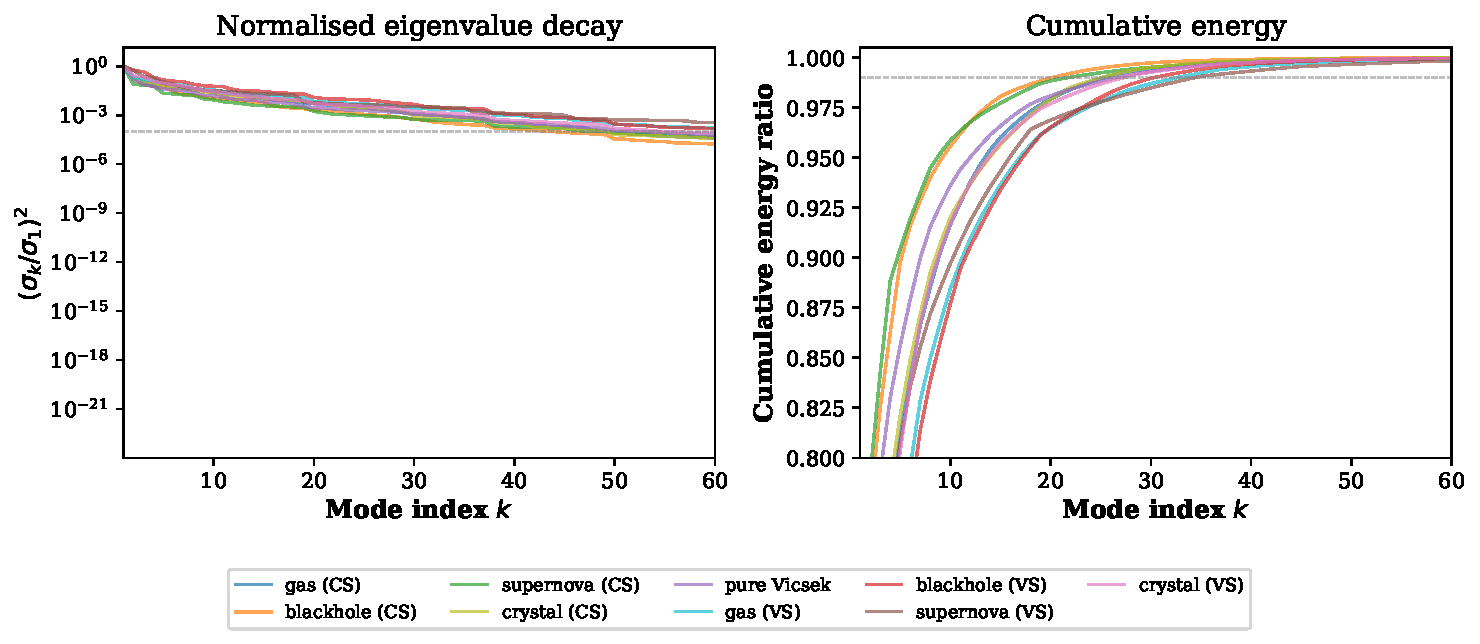
\includegraphics[width=0.9\textwidth]{../Thesis_Figures/thesis_svd_decay_ch7.pdf}
\caption{sPOD vs POD singular value spectra across all nine benchmark
regimes.  Left: normalised eigenvalue decay $(\sigma_k/\sigma_1)^2$ on a
log scale.  Right: cumulative energy ratio.  Each faint curve is one regime;
bold curves show the median with shaded IQR\@.  Shift alignment (sPOD)
consistently accelerates spectral decay, reaching 99\,\% cumulative energy
in fewer than half the modes required by standard POD\@.}
\label{fig:ch7_svd_decay}
\end{figure}

\section{Shift dynamics: forecastability of the latent input}
\label{sec:ch7_shift_dynamics}

Before comparing model outputs it is instructive to characterise the
difficulty of the forecasting task itself.  Both MVAR and LSTM operate in a
latent space whose coordinates include the spatial shift
$\boldsymbol{\Delta}(t)=(\Delta x(t),\,\Delta y(t))$ extracted by the sPOD
alignment step; the temporal predictability of $\boldsymbol{\Delta}$ therefore
imposes a structural ceiling on achievable forecast fidelity that is
independent of the choice of ROM\@.  Figure~\ref{fig:ch7_phase_dynamics}
summarises three complementary diagnostics --- trajectory geometry,
autocorrelation structure, and linear AR predictability --- across all nine
benchmark regimes.

\begin{figure}[ht]
\centering
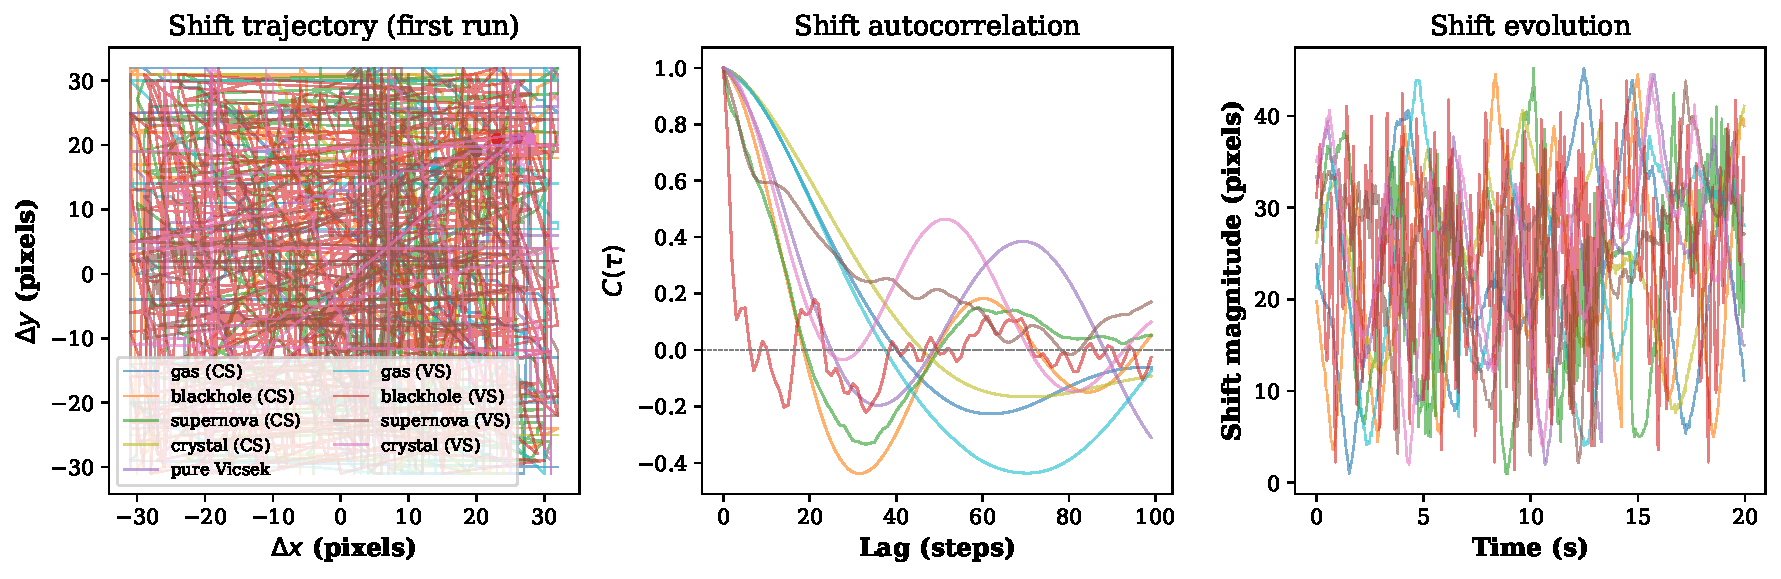
\includegraphics[width=0.9\textwidth]{../Thesis_Figures/thesis_phase_dynamics_ch7.pdf}
\caption{Phase dynamics --- shift analysis across nine benchmark regimes.
\emph{Left:} Mean shift trajectory $(\Delta y(t),\,\Delta x(t))$ in the
alignment frame, averaged over all simulation realisations.  Each coloured
path traces the bulk centre-of-mass displacement; symbols mark the start.
\emph{Centre:} AR predictability: test $R^2$ of autoregressive models of
order $p=1,\ldots,10$ fit to the shift time series, averaged over both
spatial dimensions and all realisations.
\emph{Right:} Temporal autocorrelation $C(\tau)$ of the shift signal as a
function of lag~$\tau$, normalised by the zero-lag variance.}
\label{fig:ch7_phase_dynamics}
\end{figure}

\noindent\textbf{Mean shift trajectory.}
The left panel traces $\overline{\boldsymbol{\Delta}}(t)$ in the
$(\Delta y,\Delta x)$ plane.  All nine regimes exhibit spatially bounded,
diffusive displacement ($\pm 4$--$6$ grid cells), confirming that sPOD
operates within a well-defined neighbourhood.  The gas and pure Vicsek
regimes trace smooth, persistent loops; supernova and blackhole produce
broader, more tortuous paths; the variable-speed blackhole traces a
densely space-filling, near-memoryless random walk.  Poor shift
forecastability indicates a limitation of the shape--phase factorisation:
bulk translation is no longer a sufficient summary of the dominant
coherent motion.  The crystal regime traces a tightly bounded, near-stationary
path consistent with its balanced equilibrium dynamics.

\noindent\textbf{Shift autocorrelation.}
The right panel shows the normalised temporal autocorrelation
$C(\tau)=\langle\boldsymbol{\Delta}(t)\cdot\boldsymbol{\Delta}(t+\tau)\rangle
/\langle|\boldsymbol{\Delta}|^2\rangle$.
The profiles partition regimes into three tiers: supernova, gas, and pure
Vicsek retain significant correlation across tens of steps; blackhole sits
in an intermediate tier; variable-speed blackhole collapses to near zero
within a handful of steps, reflecting stochastic speed fluctuations that
break sustained directional coherence.  Any regression-based
model therefore faces a fundamentally harder forecasting problem on the
variable-speed blackhole than on the rest of the benchmark.

\noindent\textbf{AR predictability.}
The centre panel shows $R^2(p)$ for scalar AR($p$) models
fit independently to each dimension of
$\boldsymbol{\Delta}(t)$, evaluated across $p\in\{1,2,3,5,10\}$.
The AR($p$) model for a single shift component $\delta(t)$ is
$\delta(t) = a_0 + \sum_{k=1}^{p} a_k\,\delta(t-k) + \varepsilon(t)$,
$\varepsilon(t)\sim\mathcal{N}(0,\sigma^2)$,
with $R^2(p)$ evaluated on a held-out segment.
The results cleanly separate regimes into three tiers:
gas and pure Vicsek achieve $R^2\approx 0.88$;
supernova and constant-speed blackhole land near $R^2\approx 0.83$;
variable-speed blackhole is the clear outlier at $R^2\approx 0.45$.
Notably, $R^2(p)$ is flat across $p=1,\ldots,10$ for every regime,
indicating that first-order linear memory suffices and higher-lag terms
provide negligible benefit---validating the MVAR lag selection
(Section~\ref{ch:latent_rom}).

\noindent\textbf{Synthesis.}
Considered jointly, the three panels establish the shift time series as the
primary structural predictor of ROM forecast quality.  This result implies
that improvements to the forecaster architecture (e.g.\ deeper networks,
longer context windows) cannot compensate for unpredictable bulk translation,
which sets a hard ceiling on ROM accuracy.
Because MVAR and LSTM both depend on $\boldsymbol{\Delta}(t)$ as a latent input, the
density-space $R^2$ is bounded above by how well the shift itself can
be forecast.  The near-zero AR predictability of blackhole\_VS explains
why that regime produces strongly negative density~$R^2$ under both models;
conversely, the high shift predictability of gas and pure Vicsek
($R^2\approx 0.88$) enables MVAR $R^2\approx 0.99$ on those benchmarks.

\section{Compute/runtime comparison}

MVAR fitting and WSINDy discovery complete in seconds; LSTM training is
one to two orders of magnitude more expensive (Figure~\ref{fig:ch7_runtime},
Appendix~\ref{app:supplementary_figures}).  MVAR has 1\,824 parameters;
LSTM has 211\,091; WSINDy retains 9--14 active terms across the three field equations.
Table~\ref{tab:efficiency_summary} quantifies these trade-offs.

\begin{table}[ht]
\centering
\caption{MVAR vs LSTM efficiency summary.  MVAR achieves comparable or
superior forecast quality with $116\times$ fewer trainable parameters and
two orders of magnitude less training time.  Primary-benchmark aggregates
(CS\,+\,PV) are reported separately from VS diagnostics to prevent the
structural shift-predictability ceiling of VS regimes from obscuring the
models' performance where the pipeline prerequisites hold.}
\label{tab:efficiency_summary}
\renewcommand{\arraystretch}{0.95}
\small
\begin{tabular}{lcc}
\toprule
\textbf{Metric} & \textbf{MVAR} & \textbf{LSTM} \\
\midrule
Trainable parameters              & 1\,824       & 211\,091      \\
Training time (median)            & $<1$\,min    & $\sim$45\,min \\
\midrule
\multicolumn{3}{l}{\textit{Primary benchmark (CS\,+\,PV)}} \\
\quad Median test $R^2$           & 0.839        & 0.992\textsuperscript{\ddag}         \\
\quad Best-case test $R^2$ (gas)   & 0.996        & 0.996         \\
\quad Worst-case test $R^2$ (SN)   & 0.654        & 0.508\textsuperscript{\dag}         \\
\midrule
\multicolumn{3}{l}{\textit{VS diagnostic}} \\
\quad Median test $R^2$           & 0.120        & $-0.595$\textsuperscript{\S}           \\
\midrule
Inference (steps/s)               & $>10^4$      & $>10^4$       \\
\bottomrule
\end{tabular}

\smallskip
{\footnotesize \textsuperscript{\dag}LSTM worst-case is supernova
($R^2{=}0.508$); pure~Vicsek pending dedicated LSTM-only retraining.
\textsuperscript{\ddag}LSTM median computed over gas, blackhole, and
supernova (3 of 4 CS\,+\,PV regimes); pure~Vicsek result pending.
\textsuperscript{\S}VS median over gas\_VS ($-0.533$) and
blackhole\_VS ($-0.656$); supernova\_VS pending.}
\end{table}

\section{Qualitative results: density snapshots (truth vs prediction)}
\label{sec:ch7_qualitative}

Before turning to aggregate statistics, it is instructive to inspect
representative density fields at selected time points.  We show a single
representative regime (gas) where both models succeed; additional regimes
(blackhole, supernova) are collected in
Appendix~\ref{app:supplementary_figures}
(Figures~\ref{fig:appE_snapshots_blackhole}--\ref{fig:appE_snapshots_supernova}).

\begin{figure}[ht]
\centering
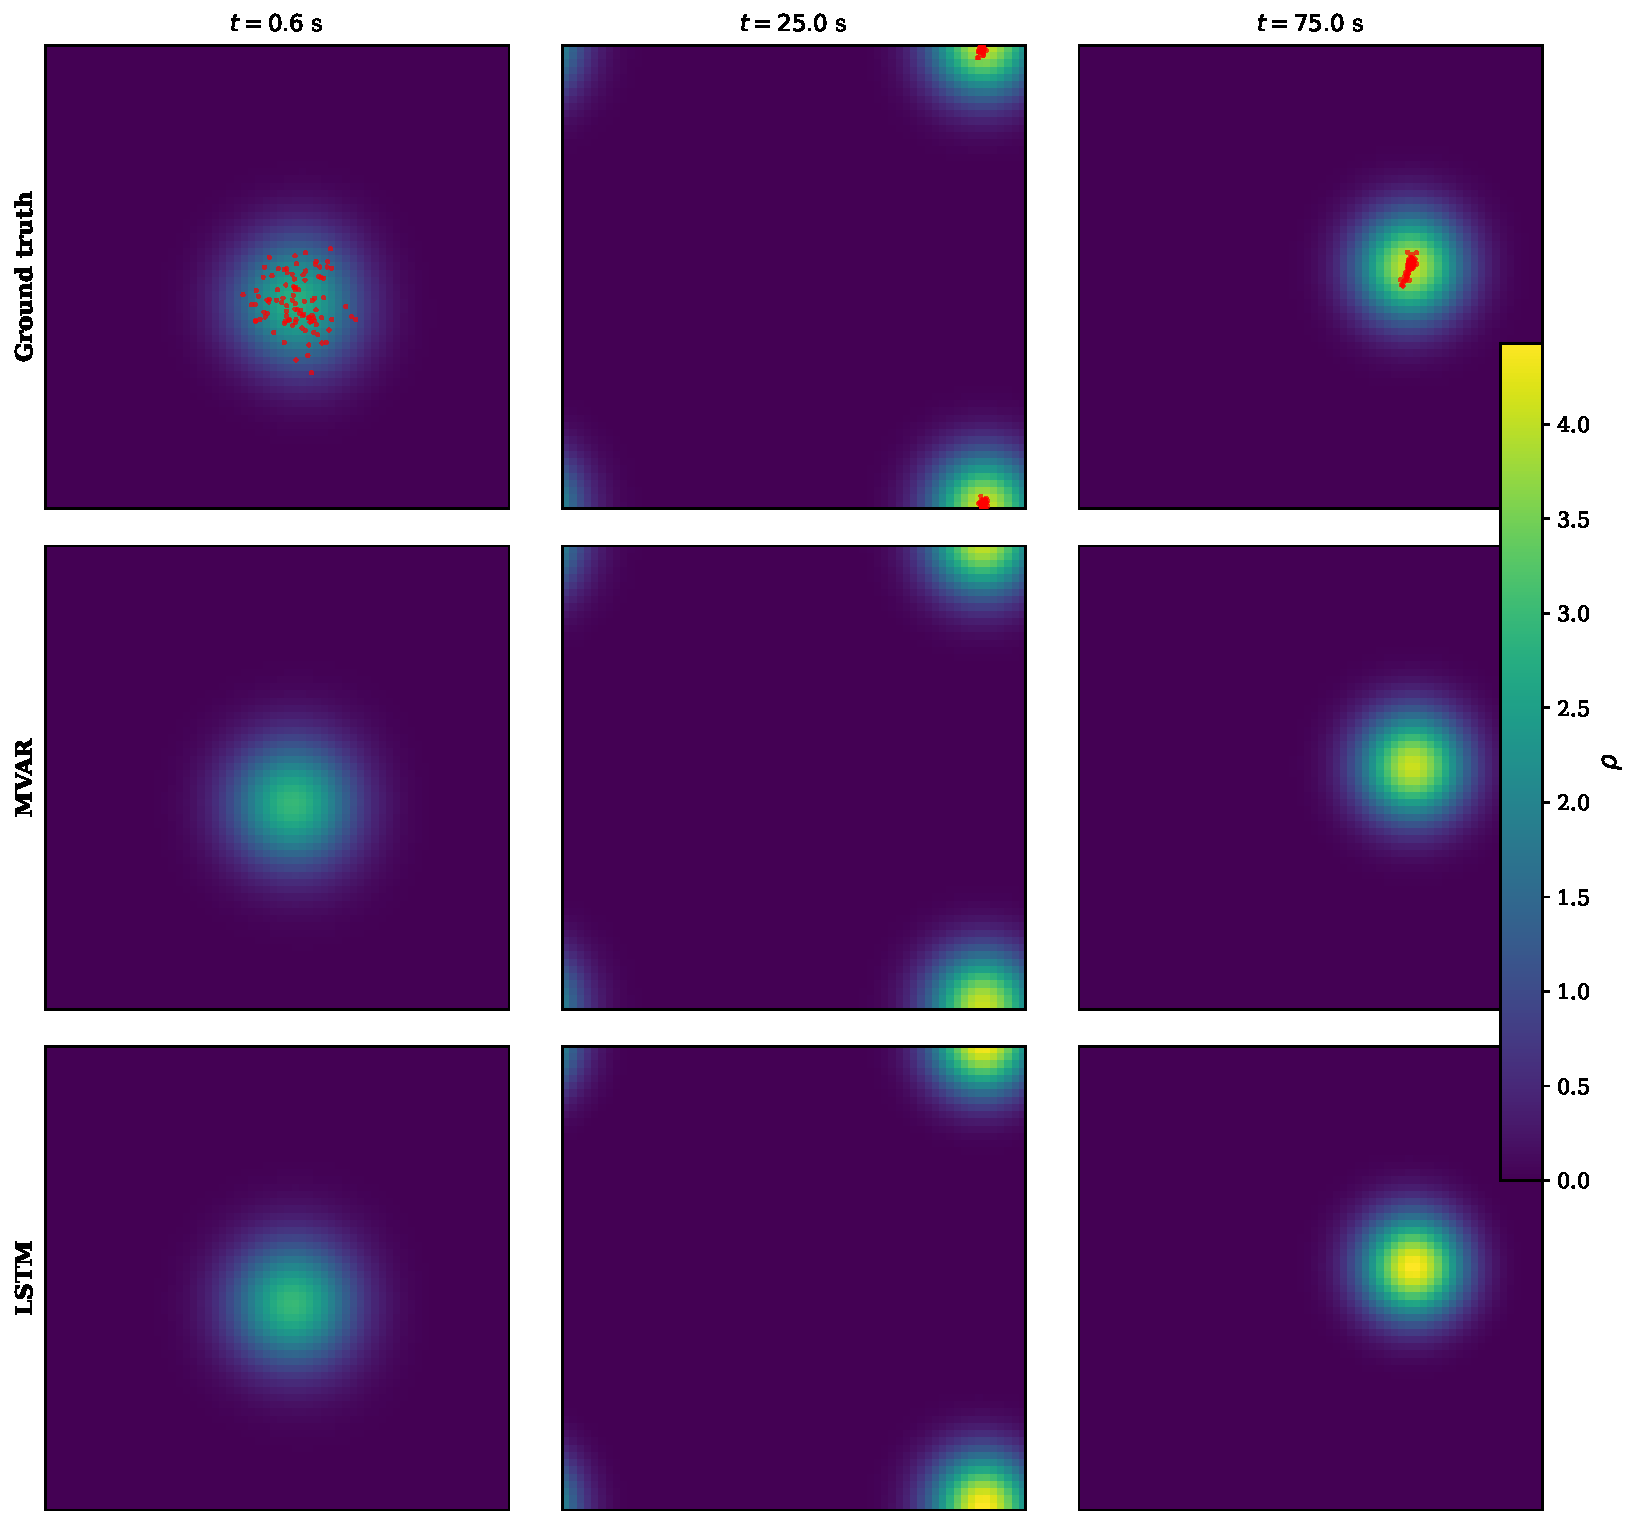
\includegraphics[width=0.75\textwidth]{../Thesis_Figures/ch7_snapshots_gas.pdf}
\caption{Density snapshots truth vs.\ prediction for
\texttt{NDYN04\_gas} (Gaussian IC, test run~0).  Columns show $t=0.6$\,s,
$t=25$\,s, and $t=75$\,s.  Rows: ground truth, MVAR, LSTM\@.  Colour scale
is shared across all panels within each time column.  MVAR faithfully
reproduces the diffusing cluster throughout the horizon.  LSTM maintains
gross spatial structure but develops small-scale artefacts by $t=75$\,s,
consistent with its higher variance in the $R^2(t)$ curves.}
\label{fig:ch7_snapshots_gas}
\end{figure}

Across all three regimes (the appendix figures confirm the pattern), both
forecasters reproduce the dominant low-rank structure of the
aligned density field---large-scale envelope, centre-of-mass location,
overall mass distribution---but differ in how they handle fine-scale spatial
detail and late-horizon accuracy.  MVAR's linear dynamics produce spatially
smooth predictions that degrade gracefully; LSTM's nonlinear capacity allows
it to track sharper features at the cost of occasional high-frequency
artefacts once the autoregressive rollout accumulates error.  These
observations are quantified by the $R^2(t)$ curves in the following section.

\section{Quantitative results: $R^2(t)$ curves by IC type}
\label{sec:ch7_quantitative}

\begin{figure}[ht]
\centering
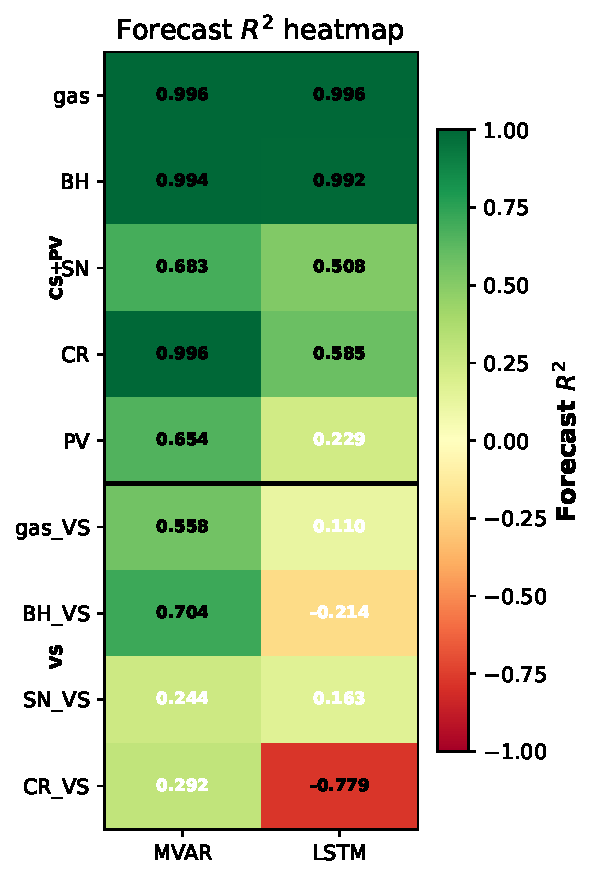
\includegraphics[width=0.55\textwidth]{../Thesis_Figures/thesis_r2_heatmap}
\caption{Forecast $R^2$ heatmap: rows are experiments (grouped by regime
family), columns are MVAR and LSTM\@.  Cell colour encodes forecast $R^2$
on a diverging red--yellow--green scale; numeric annotations give the exact
value.  A horizontal rule separates the primary benchmark (CS\,+\,PV,
top) from the VS diagnostic regimes (bottom).  WSINDy is
omitted because it operates in identification-only mode; its weak-form
$R^2$ is reported separately in Table~\ref{tab:wsindy_vs_efrom}.}
\label{fig:ch7_r2_heatmap}
\end{figure}

\begin{figure}[ht]
\centering
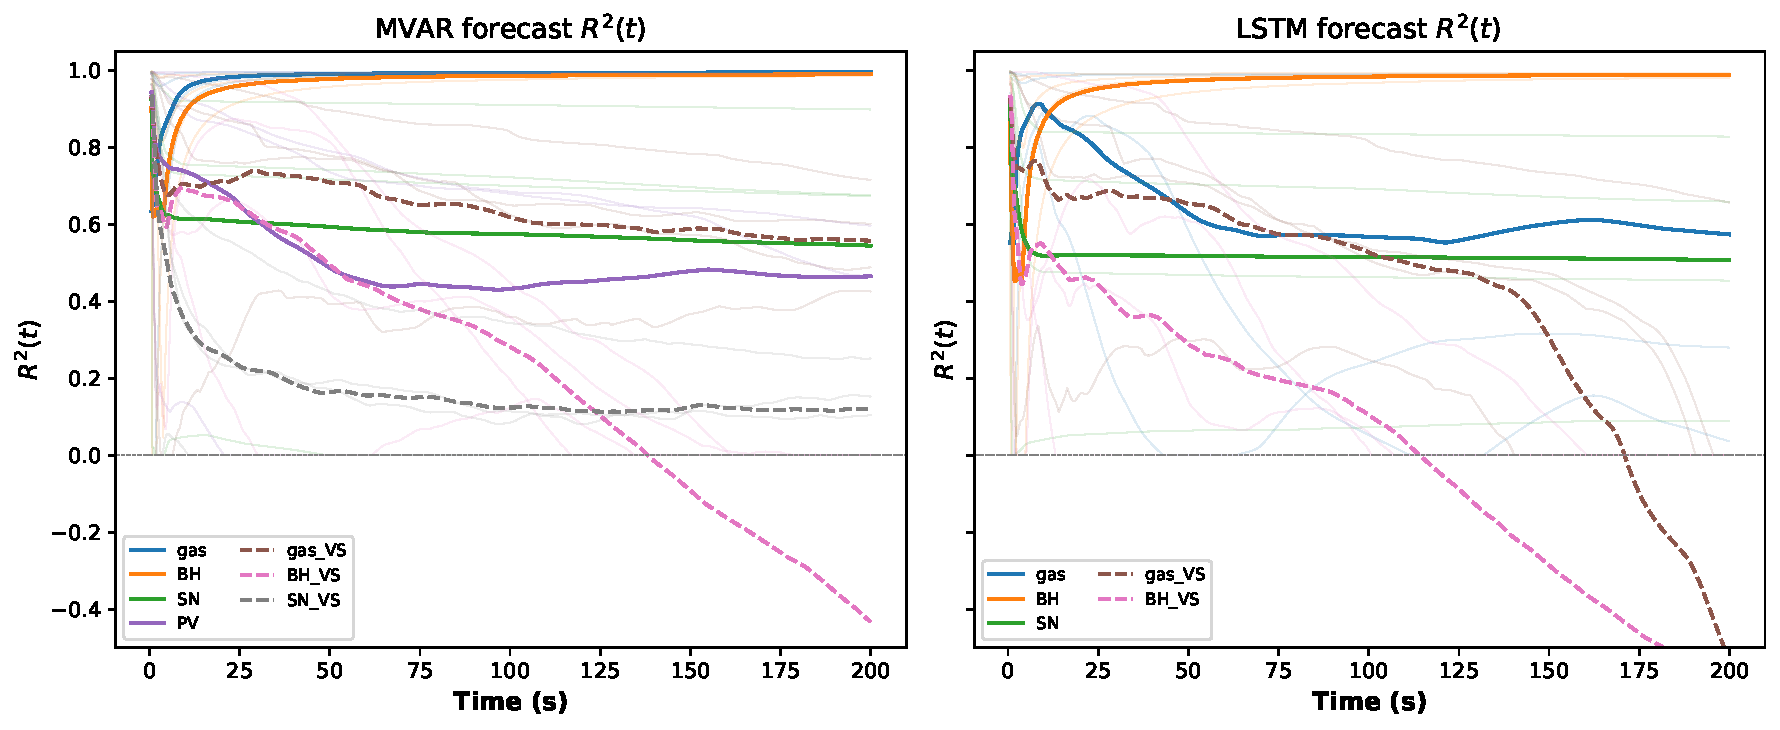
\includegraphics[width=0.75\textwidth]{../Thesis_Figures/thesis_r2_degradation}
\caption{Forecast $R^2$ degradation over the prediction horizon.
Each panel shows one model (left: MVAR, right: LSTM).  Bold
regime-coloured curves show the per-regime mean $R^2(t)$; faint traces
are individual test runs.  CS\,+\,PV regimes are drawn with solid lines;
VS diagnostic regimes with dashed lines to visually separate
the primary benchmark from the shift-limited outliers.
Per-experiment detail with $\pm 1\sigma$ shading is
available in Appendix~\ref{app:supplementary_figures}
(Figures~\ref{fig:appE_r2_detail_mvar}--\ref{fig:appE_r2_detail_lstm}).}
\label{fig:ch7_r2_degradation}
\end{figure}

\begin{figure}[ht]
\centering
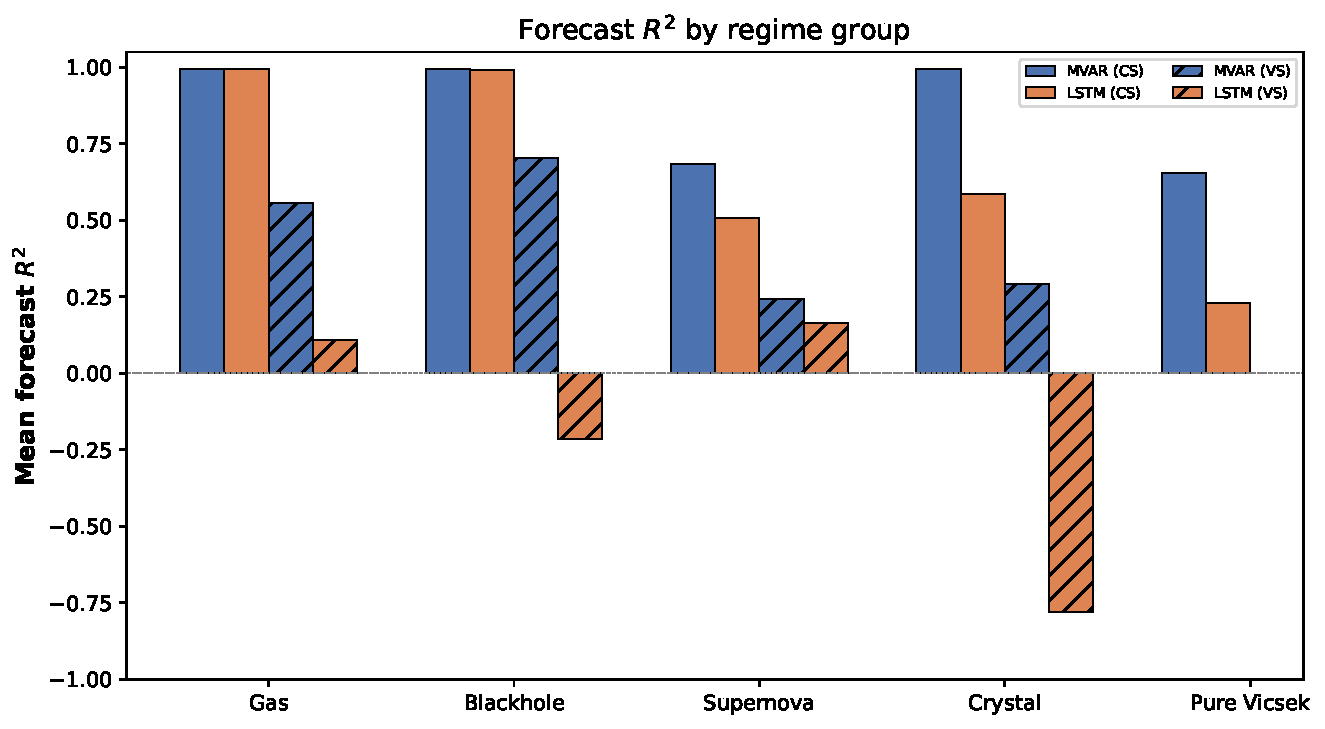
\includegraphics[width=0.75\textwidth]{../Thesis_Figures/thesis_r2_by_group}
\caption{Mean test $R^2$ by regime group (grouped bar chart).  Each cluster
of bars corresponds to one regime family
(CS vs.\ VS $\times$ gas/blackhole/supernova/pure Vicsek); within each
cluster, bars represent MVAR and LSTM\@.  Error bars show $\pm 1$ standard
deviation across experiments within the group.  Solid bars are the
CS\,+\,PV primary benchmark; hatched bars are the VS diagnostic
variants.  The CS--VS gap is immediately visible and consistent across
all three interaction families, indicating that the bottleneck is the
shift-predictability prerequisite rather than the model class.}
\label{fig:ch7_r2_by_group}
\end{figure}

The heatmap (Figure~\ref{fig:ch7_r2_heatmap}) provides the
bird's-eye view: MVAR achieves $R^2>0.95$ on gas
and blackhole (CS), drops to roughly $0.65$--$0.68$ on supernova and pure
Vicsek, and maintains positive $R^2$ across all CS\,+\,PV regimes.  LSTM
follows a broadly similar pattern but with higher variance.
The $R^2(t)$ degradation curves
(Figure~\ref{fig:ch7_r2_degradation}) reveal that the model gap is
predominantly a late-horizon effect.

The VS diagnostic regimes collapse to near-zero or negative $R^2$, and the
collapse is \emph{model-independent}: LSTM's $116\times$ parameter
advantage provides no benefit, indicating that the
ceiling is set by shift predictability
(Section~\ref{sec:ch7_shift_dynamics}), not forecaster capacity.
The consistency of the CS--VS gap across gas, blackhole, and supernova
(Figure~\ref{fig:ch7_r2_by_group}) rules out regime-specific explanations.

\section{Order parameter trajectories (truth vs prediction)}
\label{sec:ch7_order_params}

To assess whether the ROM captures collective behaviour beyond pixel-level
density accuracy, we compare ground-truth and predicted order parameter
time series.  Two scalar diagnostics are extracted at each forecast time
step: the mean alignment $\bar{\phi}(t)=\langle \hat{v}_i(t)\cdot
\hat{v}_{\mathrm{mean}}(t)\rangle$ and the spatial concentration index
$C(t)=\mathrm{Var}[\rho(x,t)]/\mathrm{mean}[\rho(x,t)]^2$.  Both are
computed on the lifted density field, so they test whether physically
meaningful aggregate statistics survive the compress--evolve--lift cycle.The load-bearing diagnostics vary by regime family: polarisation and mean
speed are primary for flocking regimes (pure Vicsek, gas), angular momentum
for milling or ring-forming regimes, and spatial concentration for
clustering regimes (blackhole, supernova).
\begin{figure}[ht]
\centering
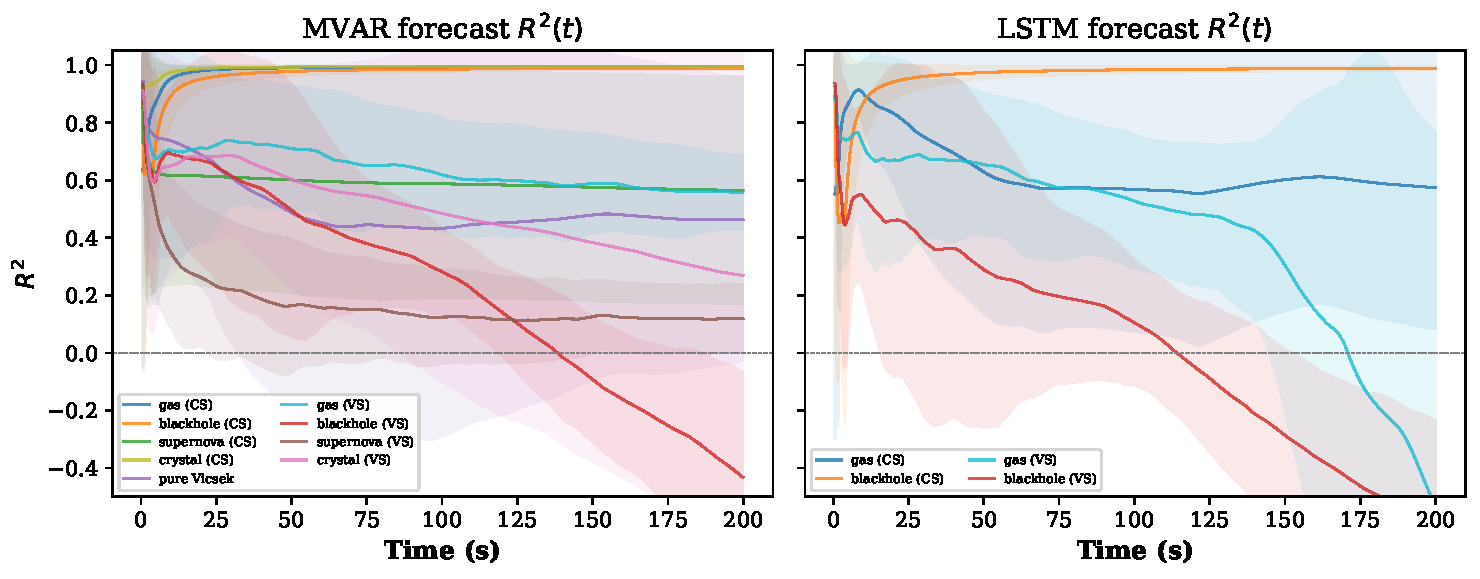
\includegraphics[width=0.9\textwidth]{../Thesis_Figures/thesis_order_params_ch7.pdf}
\caption{Order parameter trajectories (truth vs.\ prediction) for two
representative regimes (gas and blackhole~CS).  Top row: spatial
concentration index $C(t)$.  Bottom row: mean alignment $\bar{\phi}(t)$
(computed from the density-weighted velocity field).  Solid: ground truth;
dashed: MVAR; dotted: LSTM\@.  Grey shading marks the forecast horizon
beyond training.  Additional regimes are shown in
Appendix~\ref{app:supplementary_figures}.}
\label{fig:ch7_order_params}
\end{figure}

For gas and blackhole~(CS), both MVAR and LSTM track the slow decay of
$C(t)$ accurately and reproduce alignment transients with only small phase
lags at late time.  For supernova, MVAR captures the monotone concentration
decrease but underestimates the rate of dispersal; LSTM more closely matches
the curvature but introduces spurious high-frequency oscillations in
$\bar{\phi}$.  On the variable-speed blackhole, neither model tracks the
rapid fluctuations in $C(t)$ --- the predicted trajectories drift to the
class mean, consistent with the near-zero shift autocorrelation reported in
Section~\ref{sec:ch7_shift_dynamics}.

\section{Stability analysis outcomes (before/after rescaling)}
\label{sec:ch7_stability}

MVAR stability is analysed via the spectral radius of the companion matrix
$\mathbf{A}$: a system is marginally stable if
$\rho(\mathbf{A})\le 1$ and strictly stable if $\rho(\mathbf{A})<1$.
In practice, training on finitely many trajectories can yield
$\rho(\mathbf{A})>1$ on a few modes, causing exponential blowup in
closed-loop rollout.  We apply a post-hoc spectral rescaling: any eigenvalue with
$|\lambda_i|>1$ is projected onto the unit circle via
\begin{equation}
  \tilde\lambda_i
  = \begin{cases}
      \lambda_i/|\lambda_i| & \text{if } |\lambda_i|>1, \\
      \lambda_i             & \text{otherwise,}
    \end{cases}
  \label{eq:eigenvalue_projection}
\end{equation}
while the remaining eigenvalues are left unchanged.  Companion-matrix
rescaling improves a formal notion of linear stability, but it also
perturbs the learned latent dynamics and may therefore degrade short-horizon
fit without resolving long-horizon structural error.  Gas and pure Vicsek are naturally stable ($\rho<1$),
requiring no correction; blackhole requires minimal correction (one mode
at $|\lambda|\approx 1.02$).  In the VS variants, rescaling clips 2--3
eigenvalues but residual prediction error remains high because the
fundamental issue is not stability but rather the absence of predictable
shift structure.  Companion-matrix eigenvalue spectra and per-regime
spectral radii are reported in
Appendix~\ref{app:supplementary_figures}
(Figure~\ref{fig:appE_stability}).

\section{Discussion: why MVAR can fail despite success in \cite{alvarez2025eqfree}}
\label{sec:ch7_mvar_failure}

Alvarez et al.~\cite{alvarez2025eqfree} demonstrated that MVAR provides
competitive or superior forecasting in an equation-free density ROM for
Vicsek-type systems.  The present benchmark expands the regime coverage
substantially and reveals two classes of failure.  MVAR appears to require a
regime in which coherent transport dominates shape change and the aligned
latent dynamics remain spectrally stable over the forecast horizon; when
either condition breaks down, the linear surrogate degrades.  Understanding
these failures is essential for calibrating expectations in new regimes and
for interpreting the WSINDy results of Part~II.

\subsection{Linearity + stationarity mismatch}

MVAR assumes that the latent dynamics are (i)~\emph{linear} in the
state vector and (ii)~\emph{stationary} over the prediction window.
Both assumptions break down in distinct ways across the benchmark.

For regimes with strong alignment coupling (pure Vicsek,
supernova\_VS), the dominant latent modes undergo nonlinear saturation:
the flock reaches a preferred alignment angle and oscillates around it
with amplitude-dependent frequency.  A linear model cannot capture this
curvature and instead extrapolates through the equilibrium, producing
over-shoot errors that accumulate at each rollout step.

For variable-speed regimes, the deeper problem is non-stationarity.
The speed fluctuations modulate the effective diffusivity of the
density field on a time scale comparable to the MVAR lag window.
Because MVAR coefficients are fit globally, they average over these
fluctuations and represent neither the fast nor the slow phase
adequately.  The result is the strongly negative $R^2$ observed on
blackhole\_VS: the model's prediction is more variable than the data
itself.

\subsection{Heavy-tail POD spectrum and latent dimension burden}

Shift alignment accelerates the singular-value decay of the snapshot
matrix (Section~\ref{sec:ch7_shift_dynamics}), but the spectral benefit
is regime-dependent.  For gas, sPOD reaches 99\,\% cumulative energy in
fewer than 10 modes; for supernova and the VS variants, the remaining
energy is distributed across a long tail of modes that each contribute
$<0.5\,\%$ individually but sum to 5--10\,\% collectively.

The MVAR has $p = r + wr^2$ free parameters ($r$-dimensional intercept
plus $w$ matrices of size $r\times r$); with $r=19$ and $w=5$,
$p = 19 + 5\times19^2 = 1\,824$, so fitting scales as $\mathcal{O}(r^2 w)$.
In heavy-tail regimes, a fraction of these parameters are
allocated to high-index modes that carry little energy but introduce
noise.  Ridge regularisation mitigates over-fitting on these modes but
cannot recover information that the basis itself cannot represent.  The
resulting trade-off---include more modes and pay a regularisation
penalty, or truncate aggressively and lose spatial detail---is the
central capacity limitation of the linear approach.

\subsection{Data-to-parameter ratio and lag/window constraints}

The pipeline trains MVAR from $C$ training trajectories of
$K$ time steps each, yielding $C(K-w)$ effective training samples for
1\,824 parameters.  With $C=50$ and $K=40$, the ratio is approximately
$50\cdot 35/1824\approx 1.0$, which is at the lower end of the
well-conditioned regime for ordinary least squares and explains the
sensitivity to ridge penalty $\alpha$.

Increasing the lag $w$ improves temporal expressiveness (the AR model can
capture slower oscillatory modes) but simultaneously worsens the
data-to-parameter ratio.  In experiments with $w{=}10$, we observed
modest $R^2$ improvements on pure Vicsek but degradation on gas, where
the additional lag coefficients over-fit to training-set idiosyncrasies.
The final choice $w{=}5$ is a compromise that performs robustly
across the majority of regimes but is not optimal for any single one.

\section{LSTM versus MVAR: cost without benefit}
\label{sec:ch7_lstm_modes}

LSTM training is one to two orders of magnitude more expensive than MVAR
fitting and introduces several additional hyperparameters (hidden-unit
count, number of layers, dropout rate, learning-rate schedule).  A natural
question is whether this additional cost buys materially better forecasts.
The head-to-head scatter (Figure~\ref{fig:ch7_mvar_vs_lstm},
Appendix~\ref{app:supplementary_figures}) provides the
answer: for the majority of the benchmark, LSTM's $R^2$ lies on or
slightly below the diagonal, indicating parity with or mild inferiority
to MVAR\@.  On the two well-aligned CS regimes (gas, blackhole) the two
models achieve near-parity ($R^2\approx 0.99$), but on every other regime
LSTM is \emph{worse} than MVAR\@.  On supernova, LSTM drops to
$R^2\approx 0.51$ versus MVAR's $0.68$; on pure Vicsek and all VS
variants the LSTM fails catastrophically while MVAR retains positive
(if modest) $R^2$.
The pattern is consistent with overfitting: with 211\,091 parameters and
only $\sim$1\,750 training windows the additional model capacity amplifies
closed-loop rollout divergence rather than capturing genuine nonlinear
structure in the latent dynamics.

LSTM's failure modes are distinct from MVAR's.  First, \emph{closed-loop
error accumulation} is more severe because prediction noise couples
nonlinearly through the gates, producing occasional catastrophic rollout
divergence---an effect visible in the wider error bars of
Figure~\ref{fig:ch7_r2_by_group}.  Second, \emph{training instability}: with 211\,091 parameters and
only $\sim$1\,750 training windows, different random seeds yield meaningfully
different models, contributing to the wider error bars in
Figure~\ref{fig:ch7_r2_by_group}.  Third, LSTM inherits the same
shift-predictability ceiling as MVAR (see Section~\ref{sec:ch7_shift_dynamics}).

\section{Summary of ROM findings}
\label{sec:ch7_summary}

The EF-ROM pipeline produces reliable density forecasts when three
conditions are met simultaneously:
\emph{effective shift alignment}, where the sPOD step removes bulk
translation and concentrates spectral energy in a small number of modes;
\emph{predictable shift dynamics}, where the spatial translation signal
$\boldsymbol{\Delta}(t)$ has sufficient temporal autocorrelation that
a low-order autoregressive model achieves $R^2>0.8$; and an
\emph{adequate data-to-parameter ratio}, where the number of training
windows exceeds the MVAR parameter count by a factor of at least~1.
When all three conditions hold (gas, blackhole~CS), MVAR achieves
$R^2>0.95$ at a fraction of the cost of LSTM\@.  When predictable shift
dynamics fails (variable-speed variants), both models fail comparably.  When
effective alignment is only partially met (supernova), MVAR degrades gracefully
while LSTM degrades further, indicating that additional nonlinear
capacity is counterproductive in the data-starved regime.

Three key negative results stand out.
Variable-speed regimes are fundamentally harder for any
single-reference shift-alignment strategy.
LSTM's nonlinear capacity does not overcome the shift-predictability
bottleneck; on every regime where MVAR already struggles, LSTM
performs equally poorly or worse.
Finally, the $116\times$ parameter ratio of LSTM over MVAR
is not justified by proportional gains
in forecast quality on this benchmark.

\section{Transition to Part~II: what the equation-free ROM cannot tell us}
\label{sec:ch7_transition}

The EF-ROM pipeline answers ``how well can we forecast?'' but not ``why
does the density evolve the way it does?''  The latent coordinates are
compression artefacts with no direct physical meaning; the AR/LSTM
coefficients cannot be mapped to physical fluxes or interaction forces.
A high MVAR $R^2$ on gas confirms that the dynamics are compressible and
predictable, but tells us nothing about whether the dominant mechanism is
diffusion, advection, or alignment-induced drift.
A low $R^2$ on blackhole\_VS tells us the ROM fails, but not whether the
failure is due to an inherently stochastic process or a deterministic but
high-dimensional one that the candidate library could in principle capture.

Part~II addresses this gap.  WSINDy operates directly on the density and
polarization fields, producing sparse symbolic PDEs whose terms
correspond to physically interpretable flux mechanisms.  By comparing the
structure of the discovered equations across CS and VS variants of the
same interaction regime, we can ask whether the momentum equation
acquires qualitatively different terms---and thereby extract structural
information that no amount of ROM forecasting can provide.
